\PassOptionsToPackage{unicode=true}{hyperref} % options for packages loaded elsewhere
\PassOptionsToPackage{hyphens}{url}
\documentclass[12pt,ignorenonframetext,aspectratio=169]{beamer}
\IfFileExists{pgfpages.sty}{\usepackage{pgfpages}}{}
\setbeamertemplate{caption}[numbered]
\setbeamertemplate{caption label separator}{: }
\setbeamercolor{caption name}{fg=normal text.fg}
\beamertemplatenavigationsymbolsempty
\usepackage{lmodern}
\usepackage{amssymb}
\usepackage{amsmath}
\usepackage{ifxetex,ifluatex}
\usepackage{fixltx2e} % provides \textsubscript
\ifnum 0\ifxetex 1\fi\ifluatex 1\fi=0 % if pdftex
  \usepackage[T1]{fontenc}
  \usepackage[utf8]{inputenc}
\else % if luatex or xelatex
  \ifxetex
    \usepackage{mathspec}
  \else
    \usepackage{fontspec}
\fi
\defaultfontfeatures{Ligatures=TeX,Scale=MatchLowercase}






%
\fi

  \usetheme[]{iqss}






% use upquote if available, for straight quotes in verbatim environments
\IfFileExists{upquote.sty}{\usepackage{upquote}}{}
% use microtype if available
\IfFileExists{microtype.sty}{%
  \usepackage{microtype}
  \UseMicrotypeSet[protrusion]{basicmath} % disable protrusion for tt fonts
}{}


\newif\ifbibliography


\hypersetup{
      pdftitle={Production function},
        pdfauthor={Deependra Dhakal},
          pdfborder={0 0 0},
    breaklinks=true}
%\urlstyle{same}  % Use monospace font for urls







% Prevent slide breaks in the middle of a paragraph:
\widowpenalties 1 10000
\raggedbottom

  \AtBeginPart{
    \let\insertpartnumber\relax
    \let\partname\relax
    \frame{\partpage}
  }
  \AtBeginSection{
    \ifbibliography
    \else
      \let\insertsectionnumber\relax
      \let\sectionname\relax
      \frame{\sectionpage}
    \fi
  }
  \AtBeginSubsection{
    \let\insertsubsectionnumber\relax
    \let\subsectionname\relax
    \frame{\subsectionpage}
  }



\setlength{\parindent}{0pt}
\setlength{\parskip}{6pt plus 2pt minus 1pt}
\setlength{\emergencystretch}{3em}  % prevent overfull lines
\providecommand{\tightlist}{%
  \setlength{\itemsep}{0pt}\setlength{\parskip}{0pt}}

  \setcounter{secnumdepth}{0}


  \usepackage{booktabs}
  \usepackage{longtable}
  \usepackage{emptypage}
  \usepackage{array}
  \usepackage{multirow}
  \usepackage{wrapfig}
  \usepackage{float}
  \usepackage{colortbl}
  \usepackage{pdflscape}
  \usepackage{tabu}
  \usepackage{threeparttable}
  \usepackage{threeparttablex}
  \usepackage[normalem]{ulem}
  \usepackage{rotating}
  \usepackage{makecell}
  \usepackage{xcolor}
  \usepackage{tikz} % required for image opacity change
  \usepackage[absolute,overlay]{textpos} % for text formatting
  \usepackage[utf8]{inputenc}
  \usetikzlibrary{mindmap}

  % this font option is amenable for beamer
  \setbeamerfont{caption}{size=\tiny}


%% IQSS overrides
\iqsssectiontitle{Outline}

\AtBeginSection[]{
  \title{\insertsectionhead}
  {
    \definecolor{white}{rgb}{0.776,0.357,0.157}
    \definecolor{iqss@orange}{rgb}{1,1,1}
    \ifnum \insertmainframenumber > \insertframenumber
    \frame{
      \frametitle{\iqsssectiontitleheader}
      \tableofcontents[currentsection]
    }
    \else
    \frame{
      \frametitle{Backup Slides}
      \tableofcontents[sectionstyle=shaded/shaded,subsectionstyle=shaded/shaded/shaded]
    }
    \fi
  }
}

\AtBeginSubsection[]{}

%%


  \title[]{Production function}



  \author[
        Deependra Dhakal
    ]{Deependra Dhakal}

  \institute[
    ]{
    GAASC, Baitadi \and Tribhuwan University
    }

\date[
      \today
  ]{
      \today
        }

\begin{document}

% Hide progress bar and footline on titlepage
  \begin{frame}[plain]
  \titlepage
  \end{frame}



\hypertarget{factor-product-relationship}{%
\section{Factor-product
relationship}\label{factor-product-relationship}}

\begin{frame}{Background}
\protect\hypertarget{background}{}
\begin{itemize}
\tightlist
\item
  When concerned with resource allocation for production optimization,
  an understanding of input-output or factor-product relationship is
  important.
\item
  First, study of physical or technical relationship is important.
  Second, for decision making, application of economic choice indicators
  such as price ratio is required.
\item
  In a simple scenario, we details the physical factor-product
  relationship of a single variable resoruce and single product.
\item
  Many time resources or capacities of technical units, such as a ropani
  of land or a cow, are fixed and choice is to vary the input of only
  one factor -- such as fertilizer \alertc{OR} labor.
\item
  Other inputs such as fixed capital, buildings, implements and
  technical knowhow remain the same.
\end{itemize}
\end{frame}

\begin{frame}{}
\protect\hypertarget{section}{}
\begin{itemize}
\tightlist
\item
  Under such situation question of how much of certain input (amount of
  fertilizer or feed to a cow) to apply arises ?
\item
  This situtation is dealt by single factor-product relationships. a.k.a
  single variable production function (in a production function various
  levels of input are involved with corresponding output of the
  product).
\end{itemize}

\begin{block}{Inputs have several different names:}
\protect\hypertarget{inputs-have-several-different-names}{}
Inputs = factors = factors of production = resources = A, L, K, M

\begin{quote}
\textbf{A}: Land (Natural and biological resources, climate.)
\newline \textbf{L}: Labor (Human resources.) \newline \textbf{K}:
Capital (Manufactured resources, which include buildings, machines,
tools, and equipment.) \newline \textbf{M}: Management (The
entrepreneur, or individual, who combines the other resources into
inputs.)
\end{quote}
\end{block}
\end{frame}

\hypertarget{types-of-factor-product-relationships-production-functions}{%
\section{Types of factor-product relationships (production
functions)}\label{types-of-factor-product-relationships-production-functions}}

\begin{frame}{Types of factor-product relationships (production
functions)}
\begin{itemize}
\tightlist
\item
  There can be three types of input-output relationships in the
  production of a commodity where one input is varied and the quantities
  of all other inputs are fixed.

  \begin{enumerate}
  \tightlist
  \item
    Constant marginal rate of returns (Constant productivity)
  \item
    Increasing marginal rate of returns (Increasing productivity)
  \item
    Decreasing marginal rate of returns (Decreasing productivity)
  \end{enumerate}
\end{itemize}
\end{frame}

\begin{frame}{Contant marginal rate of returns}
\protect\hypertarget{contant-marginal-rate-of-returns}{}
\begin{itemize}
\tightlist
\item
  Each additional unit of the variable input when applied to fixed
  factors, produces an equal amount of additional product. The amount of
  product increases by the same magnitude for each additional unit of
  input.
\item
  Not a very common relationship in agriculture and holds true only for
  limited range.
\item
  Example:

  \begin{enumerate}
  \tightlist
  \item
    Addition of one acre of land (technology and other factors being
    same) will add the same amount of product.
  \item
    An addition of one tractor plus driver will do the same amount of
    work as previous tractor driver unit did.
  \end{enumerate}
\end{itemize}
\end{frame}

\begin{frame}{}
\protect\hypertarget{section-1}{}
\begin{figure}
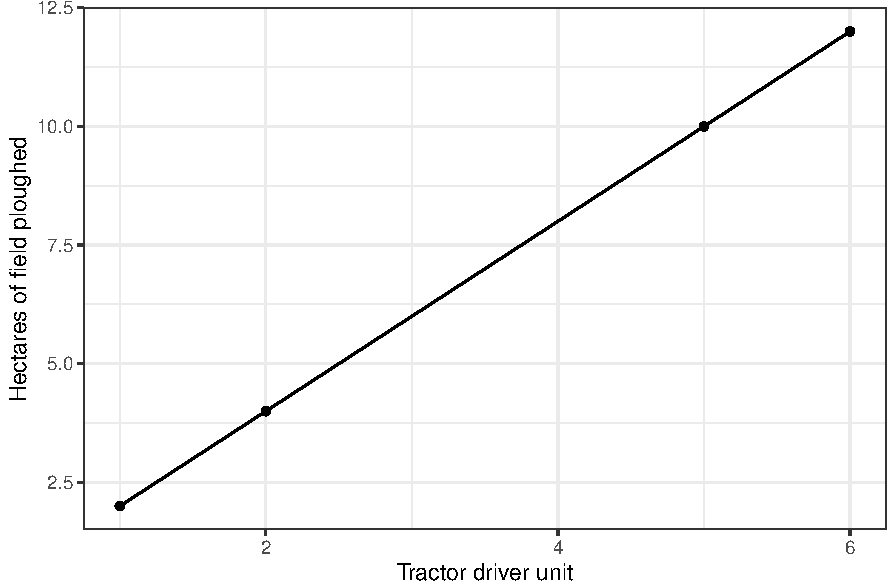
\includegraphics[width=0.7\linewidth]{04-production_function_files/figure-beamer/tractor-driver-unit-cmr-fig-1} \caption{Constant marginal rate of returns for a input-output relationship between number of tractor plus driver unit recruits and hectares of land ploughed.}\label{fig:tractor-driver-unit-cmr-fig}
\end{figure}
\end{frame}

\begin{frame}{}
\protect\hypertarget{section-2}{}
\begin{table}

\caption{\label{tab:tractor-driver-unit-cmr-tab}Constant marginal rate of returns for a input-output relationship between number of tractor plus driver unit recruits and hectares of land ploughed.}
\centering
\fontsize{6}{8}\selectfont
\begin{tabular}[t]{rrrrr}
\toprule
tractor driver unit & field ploughed & marginal tractor driver unit & marginal field ploughed & marginal rate returns\\
\midrule
1 & 2 &  &  & 2\\
2 & 4 & 1 & 2 & 2\\
5 & 10 & 3 & 6 & 2\\
6 & 12 & 1 & 2 & 2\\
\bottomrule
\end{tabular}
\end{table}
\end{frame}

\begin{frame}{Increasing marginal rate of returns}
\protect\hypertarget{increasing-marginal-rate-of-returns}{}
\begin{itemize}
\tightlist
\item
  Every additional or marginal unit of input adds more to the total
  product than the previous unit, i.e., addition to total product is at
  an increasing rate.
\item
  In actual practice, the cases of purely increasing returns are rarely
  available except, again, in very limited range.
\item
  This relationship is possible when the fixed factors of production are
  in excess capacity and addition of the small units of a variable
  resource makes more and more efficient use of fixed resources.
\item
  Example:

  \begin{enumerate}
  \tightlist
  \item
    Small quanity of wheat seed applied when other factors of production
    such as fertilizer, irrigation and other cultural practices can be
    used at high levels will give low returns.
  \end{enumerate}
\end{itemize}
\end{frame}

\begin{frame}{}
\protect\hypertarget{section-3}{}
\begin{figure}
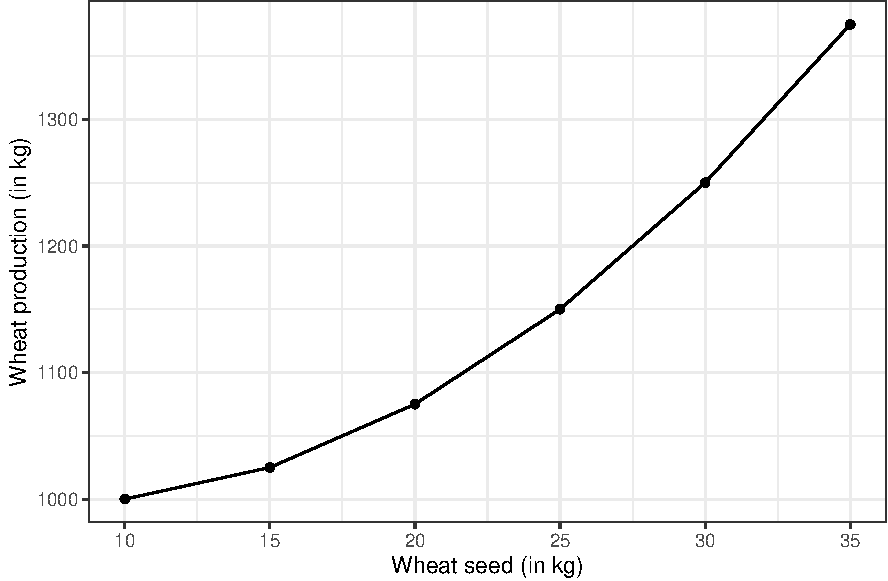
\includegraphics[width=0.7\linewidth]{04-production_function_files/figure-beamer/nitrogen-wheat-imr-fig-1} \caption{Increasing marginal rate of returns for hypothetical wheat production scenario.}\label{fig:nitrogen-wheat-imr-fig}
\end{figure}
\end{frame}

\begin{frame}{}
\protect\hypertarget{section-4}{}
\begin{table}

\caption{\label{tab:nitrogen-wheat-imr-tab}Increasing marginal rate of return for hypothetical wheat production scenario.}
\centering
\fontsize{6}{8}\selectfont
\begin{tabular}[t]{rrrrr}
\toprule
wheat seed & marginal wheat seed & wheat production & marginal wheat production & marginal rate returns\\
\midrule
10 &  & 1000 &  & \\
15 & 5 & 1025 & 25 & 5\\
20 & 5 & 1075 & 50 & 10\\
25 & 5 & 1150 & 75 & 15\\
30 & 5 & 1250 & 100 & 20\\
\addlinespace
35 & 5 & 1375 & 125 & 25\\
\bottomrule
\end{tabular}
\end{table}
\end{frame}

\begin{frame}{Decreasing marginal rate of returns}
\protect\hypertarget{decreasing-marginal-rate-of-returns}{}
\begin{itemize}
\tightlist
\item
  Each additional unit of input adds less to the total product than the
  previous unit did.
\item
  This relationship exists in almost every practical situation in
  agriculture.
\item
  Example:

  \begin{enumerate}
  \tightlist
  \item
    Response to fertilizers, insecticides, seeds, irrigation, feeds,
    etc. all show diminishing returns.
  \end{enumerate}
\end{itemize}
\end{frame}

\begin{frame}{}
\protect\hypertarget{section-5}{}
\begin{figure}
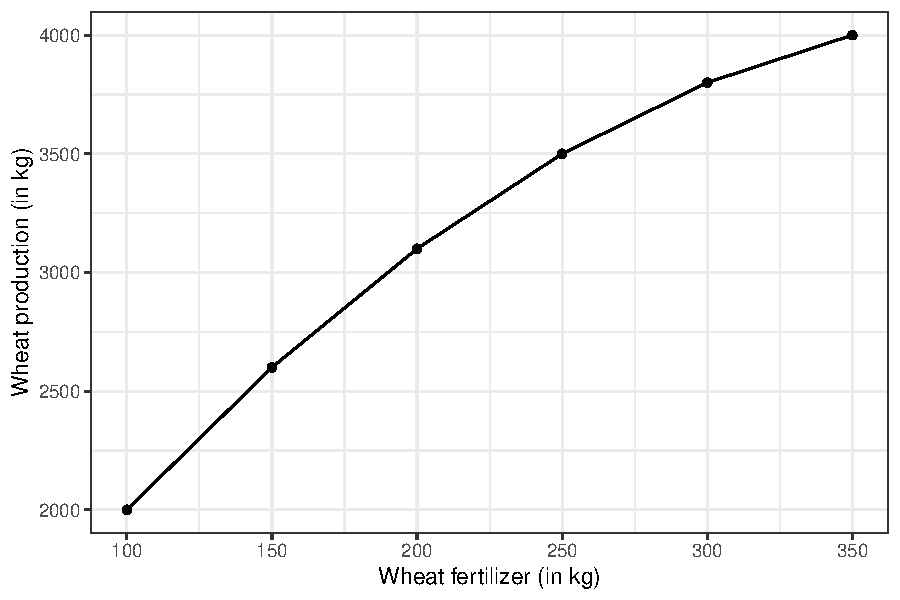
\includegraphics[width=0.7\linewidth]{04-production_function_files/figure-beamer/nitrogen-wheat-dmr-fig-1} \caption{Decreasing marginal rate of returns for hypothetical wheat production scenario.}\label{fig:nitrogen-wheat-dmr-fig}
\end{figure}
\end{frame}

\begin{frame}{}
\protect\hypertarget{section-6}{}
\begin{table}

\caption{\label{tab:nitrogen-wheat-dmr-tab}Decreasing marginal rate of return for hypothetical wheat production scenario.}
\centering
\fontsize{6}{8}\selectfont
\begin{tabular}[t]{rrrrr}
\toprule
wheat fertilizer & marginal wheat fertilizer & wheat production & marginal wheat production & marginal rate returns\\
\midrule
100 &  & 2000 &  & \\
150 & 50 & 2600 & 600 & 12\\
200 & 50 & 3100 & 500 & 10\\
250 & 50 & 3500 & 400 & 8\\
300 & 50 & 3800 & 300 & 6\\
\addlinespace
350 & 50 & 4000 & 200 & 4\\
\bottomrule
\end{tabular}
\end{table}
\end{frame}

\hypertarget{relationship-between-total-average-and-marginal-products}{%
\section{Relationship between total, average and marginal
products}\label{relationship-between-total-average-and-marginal-products}}

\begin{frame}{Physical returns or productivity relationships}
\protect\hypertarget{physical-returns-or-productivity-relationships}{}
\begin{itemize}
\tightlist
\item
  Total, average and marginal products are related.
\item
  Both the average and marginal product curves or relationships can be
  derived once total product curve has been obtained.
\end{itemize}
\end{frame}

\begin{frame}{}
\protect\hypertarget{section-7}{}
\begin{table}

\caption{\label{tab:tc-ac-mc-relationship}Relationship between total, average and marginal products}
\centering
\fontsize{6}{8}\selectfont
\begin{tabular}[t]{rrrrl}
\toprule
Units of fertilizer input & Total product (TP; Y) & Average product (AP; Y/X) & Marginal product (MP; Y/X) & Remarks\\
\midrule
\rowcolor{gray!6}  0 & 0 &  &  & \\

1 & 2 & 2.0 & 2 & \\

\rowcolor{gray!6}  2 & 5 & 2.5 & 3 & \\

3 & 9 & 3.0 & 4 & \multirow{-4}{*}{\raggedright\arraybackslash Increasing at increasing rate}\\
\cmidrule{1-5}
\rowcolor{gray!6}  4 & 14 & 3.5 & 5 & \\

5 & 19 & 3.8 & 5 & \multirow{-2}{*}{\raggedright\arraybackslash Increasing at constant rate}\\
\cmidrule{1-5}
\rowcolor{gray!6}  6 & 23 & 3.8 & 4 & \\

7 & 26 & 3.7 & 3 & \\

\rowcolor{gray!6}  8 & 28 & 3.5 & 2 & \\

9 & 29 & 3.2 & 1 & \\

\rowcolor{gray!6}  10 & 29 & 2.9 & 0 & \multirow{-5}{*}{\raggedright\arraybackslash Increasing at decreasing rate}\\
\cmidrule{1-5}
11 & 28 & 2.5 & -1 & \\

\rowcolor{gray!6}  12 & 26 & 2.2 & -2 & \multirow{-2}{*}{\raggedright\arraybackslash Decreasing at increasing rate}\\
\bottomrule
\end{tabular}
\end{table}
\end{frame}

\begin{frame}{}
\protect\hypertarget{section-8}{}
\begin{figure}
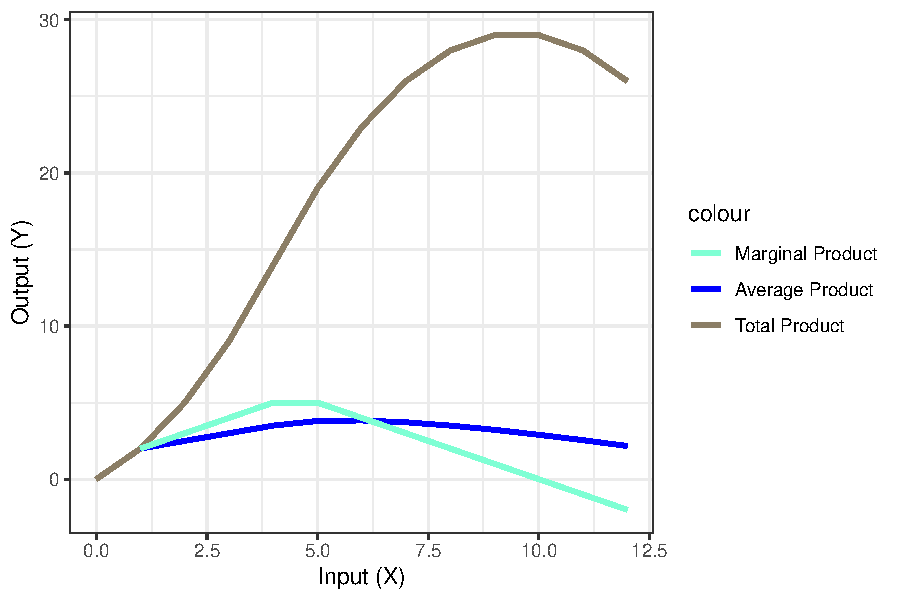
\includegraphics[width=0.7\linewidth]{04-production_function_files/figure-beamer/tc-ac-mc-relationship-plot-1} \caption{Relationship between TP, AP and MP.}\label{fig:tc-ac-mc-relationship-plot}
\end{figure}
\end{frame}

\begin{frame}{Total product (TPC) and Marginal product (MPC)}
\protect\hypertarget{total-product-tpc-and-marginal-product-mpc}{}
\begin{enumerate}
\tightlist
\item
  Since the marginal product (MP) is a measure of rate of change
  therefore:
\item
  When the Total product (TP) is increasing, the MP will be positive.
\item
  When the TP remains constant, the MP will be zero, and
\item
  When the TP decreases, the MP will be negative.
\item
  So long as MP moves upwards or increases, the TP increases at an
  increasing rate.
\item
  When the MP remains constant, the TP increases at a constant rate.
\item
  When the MP starts declining or slopes downward, the TP will be
  increasing at a decreasing rate.
\item
  At the point when MP becomes zero or when MP intersects X-axis, the
  total product will be at maximum.
\end{enumerate}
\end{frame}

\begin{frame}{Marginal product (MPC) and average product (APC)}
\protect\hypertarget{marginal-product-mpc-and-average-product-apc}{}
\begin{enumerate}
\tightlist
\item
  When the MP keeps increasing or is moving upward right from the
  beginning the Average product (AP) curve also keeps moving upward. So
  long as MP curve remains above the AP curve, the AP curve keeps
  increasing. This means when the AP is increasing, the MP must be
  greater than the average product.
\item
  As soon as the MP curve goes below the AP curve, the AP curve starts
  decreasing; i.e.~when AP is decreasing, the MP is always less than the
  AP.
\item
  When AP is equal to MP, at this point AP will be at the maximum. From
  here onward, MP will change from greater to being less than AP, the MP
  curve must therefore intersect AP curve from above at its highest
  point.
\end{enumerate}
\end{frame}

\begin{frame}{Summary of relationship between MP and AP}
\protect\hypertarget{summary-of-relationship-between-mp-and-ap}{}
\begin{enumerate}
\tightlist
\item
  When MP \textgreater{} AP, AP is increasing
\item
  When MP \textless{} AP, AP is decreasing
\item
  When MP = AP, AP is at a maximum.
\end{enumerate}
\end{frame}

\hypertarget{elasticity-of-production}{%
\section{Elasticity of production}\label{elasticity-of-production}}

\begin{frame}{Elasticity of production}
\begin{itemize}
\tightlist
\item
  The elasticity of production refers to the percentage change in output
  in response to the percentage change in input. It is be denoted by the
  symbol \(E_p\) and can be computed as:
\end{itemize}

\[
\begin{aligned}
E_p &= \frac{\frac{\Delta Y}{Y}}{\frac{\Delta X}{X}} \\
&= \frac{X}{Y}\times {\frac{\Delta Y}{\Delta X}}
\end{aligned}
\]
\end{frame}

\begin{frame}{}
\protect\hypertarget{section-9}{}
\begin{itemize}
\tightlist
\item
  Let us consider an example, given in Table
  \ref{tab:elasticity-production}.
\end{itemize}

\begin{table}

\caption{\label{tab:elasticity-production}Relationship between fertilizer input and yield of wheat.}
\centering
\fontsize{8}{10}\selectfont
\begin{tabular}[t]{rr}
\toprule
Fertilizer doses (X) & Total yield attributable to fertilizer (Y)\\
\midrule
\rowcolor{gray!6}  0 & 0\\
1 & 103\\
\rowcolor{gray!6}  2 & 174\\
3 & 223\\
\rowcolor{gray!6}  4 & 257\\
\addlinespace
5 & 281\\
\rowcolor{gray!6}  6 & 298\\
7 & 308\\
\bottomrule
\end{tabular}
\end{table}
\end{frame}

\begin{frame}{}
\protect\hypertarget{section-10}{}
As input increase from 1 to 2 units, total output increase from 103 to
174 units. Output thus increases by 71.9 percent in response to input
increase of 100 percent. The elasticity of production is therefore:

\[
\begin{aligned}
E_p &= {\frac{71.9}{100}} \\
&= 0.719
\end{aligned}
\]

Similarly, between the second and third unit of input, the elasticity
works out to be 0.56.
\end{frame}

\begin{frame}{}
\protect\hypertarget{section-11}{}
\begin{itemize}
\tightlist
\item
  Essential points to remember in elasticity analysis are:

  \begin{enumerate}
  \tightlist
  \item
    A production function with an elasticity of \(E_p = 1.0\) indicates
    constant returns throughout. This means one percent increase in
    input is always accompanied by one percent increase in output.
  \item
    The elasticity is more than 1.0 up to the point of maximum average
    product where it becomes 1.0.
  \item
    The elasticity is less than 1.0 between the points of maximum
    average product and the maximum total product.
  \item
    When it becomes less than zero, total product declines.
  \item
    When elasticity of production is 1.0, marginal and average products
    are equal. This condition holds true at only one point on the
    classical production function as shown in Figure
    \ref{fig:tc-ac-mc-relationship-plot}.
  \item
    A production function for which the elasticity is less than 1.0
    throughout all ranges of input used will indicate diminishing
    returns.
  \end{enumerate}
\end{itemize}
\end{frame}

\hypertarget{three-regions-of-production-function}{%
\section{Three regions of production
function}\label{three-regions-of-production-function}}

\begin{frame}{}
\protect\hypertarget{section-12}{}
\begin{itemize}
\tightlist
\item
  The classic production function (Figure
  \ref{fig:tc-ac-mc-relationship-plot} and Table
  \ref{tab:tc-ac-mc-relationship}) can be divided into three
  ``regions'', ``zones'', ``parts'' or ``stages'', each important from
  the standpoint of decision-making on efficient resource use.
\item
  These are (again shown in Figure
  \ref{fig:production-function-stages}):
\end{itemize}

\begin{figure}
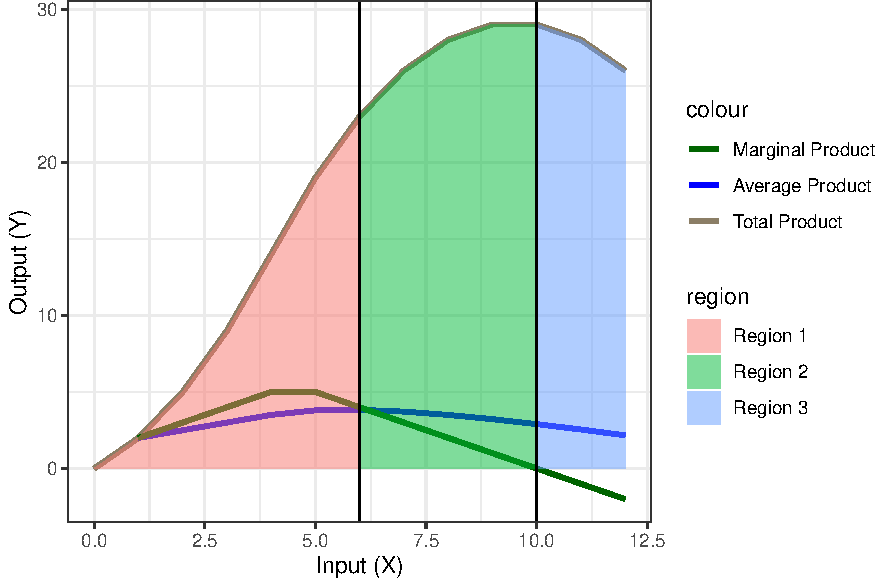
\includegraphics[width=0.7\linewidth]{04-production_function_files/figure-beamer/production-function-stages-1} \caption{Three stages of a production function.}\label{fig:production-function-stages}
\end{figure}
\end{frame}

\begin{frame}{Region 1 (irrational zone)}
\protect\hypertarget{region-1-irrational-zone}{}
\begin{itemize}
\tightlist
\item
  This region hold from the point of origin up to the point the MPP
  remains greater than APP.
\item
  The APP increases throughout this region indicating that the
  efficiency of all the units of variable input keeps increasing.
\item
  Zone terminates as soon as APP equals MPP
\item
  Notes:

  \begin{itemize}
  \tightlist
  \item
    once the farmer decides to produce, he must produce up to the level
    of input use where the APP is highest.
  \item
    the efficiency of the variable input keeps increasing throughout the
    Region 1.
  \item
    it is not reasonable to stop using an input when its efficiency on
    all units used is increasing.
  \item
    reaching to the point of highest average product is always
    profitable
  \end{itemize}
\end{itemize}
\end{frame}

\begin{frame}{Region 3 (irrational zone)}
\protect\hypertarget{region-3-irrational-zone}{}
\begin{itemize}
\tightlist
\item
  This region obtains where MPP crosses zero point and becomes negative.
\item
  Negative MPP occurs when so much excessive quanity of the variable
  input is used that total output begins to decrease.
\item
  Notes:

  \begin{itemize}
  \tightlist
  \item
    in the third region of production, the TP is decreasing.
  \item
    additional quantities of input reduce the total output in this
    region, hence it is not profitable zone even if the additional
    quantities of resources are available free of cost.
  \item
    e.g., if a farmer operates in this region -- a farmer growing local
    variety and applying fertilizer without restraint might suffer loss
    of yield due to lodging and inefficient nutrient utilization -- he
    will incurr double loss:
  \end{itemize}

  \begin{enumerate}
  \tightlist
  \item
    reduced production
  \item
    unnecessary additional cost of inputs
  \end{enumerate}
\end{itemize}
\end{frame}

\begin{frame}{Region 2 (rational zone)}
\protect\hypertarget{region-2-rational-zone}{}
\begin{itemize}
\tightlist
\item
  This region obtains when MPP is decreasing and is less than APP. In
  this region at the starting point, MPP is equal to APP and it extends
  to the point where MPP becomes zero.
\item
  The APP is also decreasing.
\item
  Within the boundaries of this region is the area of economic
  relevance. Optimum point of input-use must be somewhere in this
  rational zone.
\item
  Optimum point can, however, be located only when input and output
  prices are known.
\item
  This region of production embodies diminishing returns phase -- both
  AP and MP are decreasing.
\end{itemize}
\end{frame}

\begin{frame}{Why operate in zone II of production function ?}
\protect\hypertarget{why-operate-in-zone-ii-of-production-function}{}
\begin{itemize}
\item
  When a farmer is undertaking production on his farm, his prime
  objective is to maximize his returns. The TP curve in the production
  function shows only the total production while the MP curve represents
  the rate of returns from production. MP as a measure of farm operation
  efficiency at different level of production is useful to decide how
  much to produce with availabe quantities of input.
\item
  It is of interest to farmer that each additional unit has variable
  relations with quantity of output. One surely will not want to stop
  production when addition of input causes more increment in product
  that the earlier unit of input did. This is the case of Ist zone of
  production function. In this zone efficiency of additional input is
  increasing and the fixed factors of production are not being used upto
  their full potential. To maximize returns from production, it is
  required that input be increased.
\end{itemize}
\end{frame}

\begin{frame}{}
\protect\hypertarget{section-13}{}
\begin{itemize}
\item
  As soon as the production from additional one unit of input stops
  adding to the total product, input use beyond this level is wasteful.
  This leads to farmer incurring double loss (first from increased cost
  of input use second from reduced returns from the product itself).
\item
  However, as long as addition to total product is increasing at
  increasing rate or increasing at constant rate, or even increasing at
  decreasing rate, so that cost of additional unit of input use can be
  justified with returns from product obtained by the same additional
  unit of input, the production is carried out. The exact optimum level
  of input use, however, is determined by the price of input and output,
  both.
\end{itemize}
\end{frame}

\begin{frame}{Knowing the point of operation}
\protect\hypertarget{knowing-the-point-of-operation}{}
\begin{itemize}
\tightlist
\item
  In order to determine what level in Region 2 one should operate, one
  needs to know the product as well as the input prices. Multiplying the
  quantities of product and inputs with the respective prices we can
  convert the physical production function into revenue and cost
  functions.
\item
  Thus the optimum level of input use, will be where the additional cost
  of an input is equal to the additional revenue which the input yields.
\item
  Hence in the rational zone of production, factor-product price ratio
  will be used as a choice indicator.
\end{itemize}
\end{frame}

\begin{frame}{}
\protect\hypertarget{section-14}{}
\begin{table}

\caption{\label{tab:fp-relationship-decision-tab}Factor-product relationship and economic decision analysis.}
\centering
\fontsize{6}{8}\selectfont
\begin{tabular}[t]{>{\raggedleft\arraybackslash}p{4em}>{\raggedleft\arraybackslash}p{4em}>{\raggedleft\arraybackslash}p{4em}>{\raggedleft\arraybackslash}p{4em}>{\raggedleft\arraybackslash}p{4em}>{\raggedleft\arraybackslash}p{4em}>{\raggedleft\arraybackslash}p{4em}>{\raggedleft\arraybackslash}p{4em}>{\raggedleft\arraybackslash}p{4em}>{\raggedleft\arraybackslash}p{4em}}
\toprule
Physical input units nitrogen ropani & Physical output units ropani & Physical marginal input units & Physical marginal product units & Physical average product & Economic marginal cost unit & Economic marginal returns unit & Economic total returns & Economic total cost inputs & Economic profit\\
\midrule
0 & 2 &  &  &  &  &  & 6 & 0 & 6\\
1 & 5 & 1 & 3 & 5.0 & 4 & 9 & 15 & 4 & 11\\
2 & 9 & 1 & 4 & 4.5 & 4 & 12 & 27 & 8 & 19\\
3 & 14 & 1 & 5 & 4.7 & 4 & 15 & 42 & 12 & 30\\
4 & 21 & 1 & 7 & 5.2 & 4 & 21 & 63 & 16 & 47\\
\addlinespace
5 & 26 & 1 & 5 & 5.2 & 4 & 15 & 78 & 20 & 58\\
6 & 30 & 1 & 4 & 5.0 & 4 & 12 & 90 & 24 & 66\\
7 & 33 & 1 & 3 & 4.7 & 4 & 9 & 99 & 28 & 71\\
8 & 35 & 1 & 2 & 4.4 & 4 & 6 & 105 & 32 & 73\\
9 & 36 & 1 & 1 & 4.0 & 4 & 3 & 108 & 36 & 72\\
\addlinespace
10 & 36 & 1 & 0 & 3.6 & 4 & 0 & 108 & 40 & 68\\
11 & 35 & 1 & -1 & 3.2 & 4 & -3 & 105 & 44 & 61\\
12 & 33 & 1 & -2 & 2.8 & 4 & -6 & 99 & 48 & 51\\
\bottomrule
\end{tabular}
\end{table}
\end{frame}

\begin{frame}{}
\protect\hypertarget{section-15}{}
\begin{itemize}
\tightlist
\item
  Take for example Table \ref{tab:fp-relationship-decision-tab}, the
  price per unit of input to be Rs. 4 and price per unit of product Rs.
  3. Multiply the various quantities of product at different levels of
  input-use by Rs. 3. Assuming the producer's purchases are low enough
  not to cause the price of the input to rise, each input unit will cost
  Rs. 4. This is shown in 6th column of the Table
  \ref{tab:fp-relationship-decision-tab}.
\item
  We can see from the Table \ref{tab:fp-relationship-decision-tab} that
  the highest net revenue can be obtained when 8 units of the input are
  used yielding net revenue at Rs 73. If the producer applies less
  number of input units, say 7 units, the net revenue will be less. Here
  the returns from the last unit of input are greater than the costs,
  indicating a scope of further increasing the revenue by pushing up
  input use.
\end{itemize}
\end{frame}

\begin{frame}{}
\protect\hypertarget{section-16}{}
\begin{itemize}
\tightlist
\item
  On the other hand, if inputs are added to the point where the price of
  the input exceeds the value of the marginal product, the added costs
  go greater than the added returns.
\item
  By adding the 9th unit of input, the additional returns will be only
  Rs 3 whereas the cost of this unit of input will be the same Rs 4.
  This means it does not pay the producer to add more than 8 units of
  the input.
\item
  Optimum level of input use will thus be where the value of the
  additional product will be equal to the cost of additional input.
\end{itemize}
\end{frame}

\begin{frame}{}
\protect\hypertarget{section-17}{}
\begin{itemize}
\tightlist
\item
  We can write this condition for maximization of net revenue as:
\end{itemize}

\[
P_{Y1} \Delta Y_1 = P_{X1} \Delta X_1
\]

Where \(P_{Y1} \Delta Y_1\) is added revenue and \(P_{X1} \Delta X_1\)
is added cost.

\begin{itemize}
\tightlist
\item
  This can be written in ratio form as well.
\end{itemize}

\[
\frac{\Delta Y_1}{\Delta X_1} = \frac{P_{X1}}{P_{Y1}}
\]
\end{frame}

\hypertarget{impact-of-technological-change-on-production-function}{%
\section{Impact of technological change on production
function}\label{impact-of-technological-change-on-production-function}}

\begin{frame}{Impact of technological change on production function}
\begin{itemize}
\tightlist
\item
  Technical advances may result in such development as evolution of new
  crop varieties, breeds of animals and birds, invention of new
  fertiliers and their use methods, improved rations, new farm machinery
  etc.
\item
  So far we have made or point about production function with assumption
  that technology remains constant.
\item
  Application of different technology results in a different production
  function.
\end{itemize}
\end{frame}

\begin{frame}{}
\protect\hypertarget{section-18}{}
\begin{tikzpicture}[
  transform shape, mindmap,
  grow cyclic, 
  text width = 4.5cm, %align=flush center, %automatically formatted by mindmap
  scale=0.6, every node/.style={scale=0.6, concept, concept color=orange},
  level 1/.append style={level distance=4cm, sibling angle=120}, 
  level 2/.append style={level distance=2.5cm, sibling angle=45}]

\node{Technology}
  child {node {Impacts how ?}
    child {node {\scriptsize Replacement of old products by new ones}}
    child {node {\scriptsize Create new inputs or improve old ones}}
    child {node {\scriptsize Affect the production process}}
  }
  child {node {Types}
    child {node {\scriptsize Superior: Upward shift of production function}}
    child {node {\scriptsize Inferior: Downward shift of production function}}
  }
  child {node {General impact}
    child {node {\scriptsize Factor saving}}
    child {node {\scriptsize Yield increasing}}
    child {node {\scriptsize Both factor saving and yield increasing}}
  }
  child {node {Broader impacts}
    child {node {\scriptsize Safter growing environment and safer food}}
    child {node {\scriptsize Higher crop productivity}}
    child {node {\scriptsize Decreased  use of water, fertilizer, and pesticides}}
    child {node {\scriptsize Lower food prices}}
    child {node {\scriptsize Reduced impact on natural ecosystems}}
    child {node {\scriptsize Less runoff of chemicals into rivers and groundwater}}
    child {node {\scriptsize Increased worker safety}}
    }
;
\end{tikzpicture}
\end{frame}

\hypertarget{bibliography}{%
\section{Bibliography}\label{bibliography}}

\begin{frame}{For more information}
\protect\hypertarget{for-more-information}{}
\end{frame}




\end{document}
